\documentclass[11pt]{article}
\usepackage[utf8]{inputenc}
\usepackage[T1]{fontenc}
\usepackage{geometry, tikz, xcolor, enumitem, ragged2e}
\geometry{a4paper, margin=1.5cm}

\begin{document}

\begin{center}
\Large \textbf{\textcolor{green!50!black}{Atividade Remota: Cultura Digital – Mídias Digitais e Segurança Digital}}\\[0.3cm]
\large Professor: Jefferson
\end{center}

\vspace{0.3cm}
\large Nome: \underline{\hspace{8cm}} \quad Turma: \underline{\hspace{3cm}}

\vspace{0.5cm}

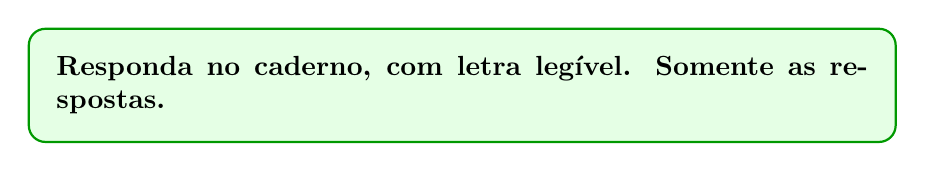
\begin{tikzpicture}
\node[rectangle, fill=green!10, rounded corners=6pt, inner sep=10pt, draw=green!60!black, thick]{
\begin{minipage}{0.85\linewidth}
\textbf{Responda no caderno, com letra legível. Somente as respostas.}
\end{minipage}
};
\end{tikzpicture}

\vspace{0.6cm}

\begin{enumerate}

\item Mídias digitais são plataformas e ferramentas online usadas para comunicação e compartilhamento de conteúdo. Elas influenciam nossa vida por facilitar o acesso à informação, à comunicação e ao entretenimento.

\item Segurança digital é o conjunto de práticas para proteger dados e informações na internet. Ela é importante para evitar golpes, invasões e uso indevido das nossas informações.

\item Devemos evitar compartilhar dados pessoais sensíveis, verificar a confiabilidade dos sites, usar senhas fortes e nunca enviar documentos pessoais em redes sociais.

\item Um vírus digital é um programa malicioso que pode danificar arquivos, roubar informações ou prejudicar o funcionamento de um computador.

\item Senhas fortes e diferentes dificultam que invasores tenham acesso às nossas contas. Se uma senha for descoberta, as outras ainda permanecerão protegidas.

\item Para identificar fake news, devemos verificar a fonte, analisar se o conteúdo possui dados confiáveis, procurar a mesma informação em meios reconhecidos e desconfiar de mensagens alarmistas.

\item Ciberbullying é a prática de agressões, humilhações ou ofensas pela internet. Podemos combatê-lo denunciando, bloqueando agressores e promovendo respeito no ambiente digital.

\item Boas práticas: manter senhas seguras, não clicar em links suspeitos, atualizar dispositivos, usar antivírus, conferir a fonte de notícias e evitar compartilhar informações sem verificar.

\end{enumerate}

\end{document}

